% !TEX encoding = UTF-8
\documentclass[a4paper,twoside,11pt]{article}
\usepackage{ccs_physiqueIIPC}
\sisetup{per-mode=reciprocal}
\documents{\logicielpython}

	%ou - (rien), par défaut si on appelle pas la commande \documents
	%ou \film{avi}
	%ou \logiciel{Java}
	%ou \pdf{NOTICE} pour spécifier un doc du type 9999TEST-NOTICE.pdf
	%ou \doc pour ''Analyse de document''
\begin{document}

\qt
	On a une interférence à deux ondes au point $M$ entre celle qui passe la lame semi-réfléchissante et qui arrive selon $y$ (je l'appellerai dans la suite l'onde 1) et celle qui se réfléchit deux fois (que j'appellerai onde 2). 
	L'intensité vaut alors 
	$$
	I(M)=I_0+I_1+2\sqrt{I_0I_1}\cos(\varphi(M))
	$$
	où $\varphi(M)=\varphi_2(M)-\varphi_1(M)$, $I_0=KA_0^2$ et $I_1=KA_1^2$ (où $K$ est le coefficient reliant intensité et amplitude).\\
	
	Concernant l'onde directe 1 (selon $y$), tous les points du plan ont même phase. On a donc $\varphi_1(O)=\varphi_1(M)$.\\
	Pour l'onde 2, en considérant le point $H$ qui est le projeté orthogonale de $M$ sur le rayon passant par $O$ on a d'après le théorème de Malus $(SH)=(SO)$. En déduit alors 
	$$
	\varphi_2(M)-\varphi_2(O)=\dfrac{2\pi }{\lambda}((SM)-(SO))=\dfrac{2\pi }{\lambda}((SH)+(HM)-(SO))=\dfrac{2\pi }{\lambda}HM=\dfrac{2\pi }{\lambda}x\sin(\theta)
	$$
	\begin{center}
		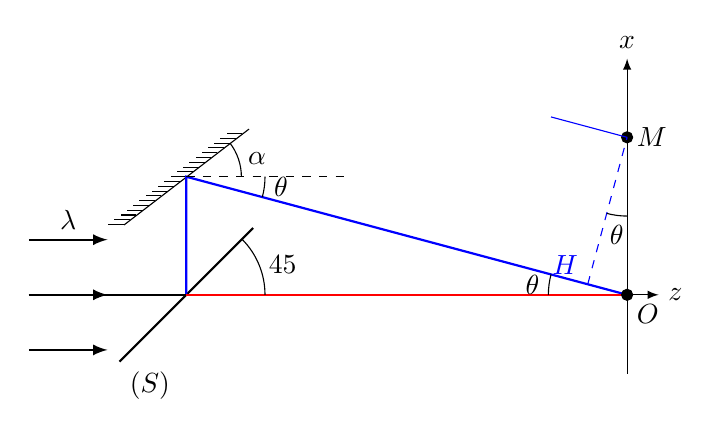
\begin{tikzpicture}
			\draw[thick] (45:-1.2)node[anchor=north west]{$(S)$}--(45:1.2);
			\draw[-latex] (-2,0)--(6,0)node[right]{$z$};
			\draw[-latex] ({1.5/tan(15)},-1)--++(0,4)node[above]{$x$};
			\draw (0,1.5)++(37.2:1)--++(37.5:-2);
			\foreach \x in {-1,-.9,...,1}
			{
				\draw (0,1.5)++(37.5:\x)--++(-.2,0);
			}
			\draw[thick,blue] (0,0)--(0,1.5)--++(-15:{1.5/sin(15)});
			\draw[thick,red] (0,0)--({1.5/tan(15)},0);
			\draw[fill] ({1.5/tan(15)},0)node[anchor=north west]{$O$}circle(2pt) ({1.5/tan(15)},2)node[right]{$M$}circle(2pt);
			\draw[thick] (-2,0)--(0,0);
			\draw[thick,-latex] (-2,-.7)--++(1,0);
			\draw[thick,-latex] (-2,0)--++(1,0);
			\draw[thick,-latex] (-2,.7)--node[above]{$\lambda$}++(1,0);
			\draw (1,0)arc[start angle=0,end angle=45,radius=1cm]node[right,pos=.5]{$\SI{45}{\degree}$};
			\draw[dashed] (0,1.5)--++(2,0);
			\draw (.7,1.5)arc[start angle=0,end angle=37.7,radius=.7cm]node[right,pos=.5]{$\alpha$};
			\draw[dashed,blue] ({1.5/tan(15)},0)++(-15:{-2*sin(15)})node[anchor=south east]{$H$}--({1.5/tan(15)},2);
			\draw[blue] ({1.5/tan(15)},2)--++(-15:-1);
			\draw (0,1.5)++(-15:1)arc[start angle=-15,end angle=0,radius=1]node[right,pos=.5]{$\theta$};
			\draw ({1.5/tan(15)},0)++(-1,0)arc[start angle=180,end angle=165,radius=1]node[left,pos=.5]{$\theta$};
			\draw ({1.5/tan(15)},2)++(0,-1)arc[start angle=-90,end angle=-105,radius=1]node[below,pos=.5]{$\theta$};
		\end{tikzpicture}
	\end{center}
	Il reste alors à déterminer $\theta$... L'angle entre les deux rayons bleus passant par le miroir vaut $\beta=\pi/2-\theta$ et on a 
	$$
	\pi=2\alpha+2\theta+\beta=2\alpha+\theta+\pi/2\Rightarrow \theta=\pi/2-2\alpha=\varepsilon
	$$
	D'où finalement 
	$$
	\varphi(M)=\varphi_2(M)-\varphi_1(M)=\varphi_2(M)-\varphi_2(O)+\underbrace{\varphi_2(O)-\varphi_1(O)}_{=O\text{ par Hyp}}+\underbrace{\varphi_1(O)-\varphi_1(M)}_{=0}=\dfrac{2\pi }{\lambda}x\sin(\theta)\simeq \dfrac{2\pi }{\lambda}x\varepsilon
	$$
	et l'intensité vaut 
	$$
	I(x,y)=I_0+I_1+2\sqrt{I_0I_1}\cos\left( \dfrac{2\pi }{\lambda}x\varepsilon\right) 
	$$

\qt L'interfrange correspond à la période du $\cos$ soit $\boxed{i=\dfrac{\lambda}{\varepsilon}}$... 


\qt  bien entendu le contraste vaut 
$$
V=\dfrac{2\sqrt{I_0I_1}}{I_0+I_1}=\dfrac{2\sqrt{r}}{1+r^2}
$$
Il est optimal pour $r=1$ et vaut dans ce cas 1 ...

\qt En suivant les indications
$$
n=K(I_0+I_1+2\sqrt{I_0I_1}\cos\left( \dfrac{2\pi }{\lambda}x\varepsilon\right) )=n_0+\Delta n\cos\left(qx\right) 
$$
avec $n_0=K(I_0+I_1)$, $\Delta n=2K\sqrt{I_0I_1}$ et $q= \dfrac{2\pi }{\lambda}\varepsilon$.\\
La concentration va s'homogénéiser sous l'effet de la diffusion pour tendre vers $n_0$
\qt Il s'agit de l'équation de diffusion sans terme source 
$$
\dpp{n}{t}=D\dps{n}{x}
$$
\qt On a comme indiqué précédemment 
$$
n_0=K(I_0+I_1)\quad \quad f(x)=\Delta n\cos(qx)
$$

En injectant la séparation des variables, on trouve 
$$
g'=-Dq^2g\Rightarrow g=\exp(-Dq^2t)
$$



\qt On voit que pour chaque valeur de $\varepsilon$ (ou valeur de $q$), $g(t)$ décroît exponentiellement. Il faut donc tracer 
$$
\ln(g(t))=f(t)
$$
et faire un ajustement linéaire pour en déduire $k=Dq^2$ par régression linéaire. \\
On peut alors $k=f(q^2)$ et on s'attend à trouver une droite de coefficient directeur $D$.

\qt cf script Python. On trouve après les traitements évoqués précédemment $D=\SI{2.5e-13}{\m\squared\per\s}$

Si un candidat est pénible, on peut toujours discuter l'incertitude sur $\varepsilon$ et lui demander un Monte Carlo pour trouver l'incertitude sur $D$. Ca lui apprendra !
\end{document}